\documentclass[conference]{IEEEtran}
\IEEEoverridecommandlockouts

\usepackage[utf8]{inputenc}
\usepackage[T1]{fontenc}
\usepackage[brazil]{babel}
\usepackage{cite}
\usepackage{amsmath,amssymb,amsfonts}
\usepackage{algorithm}
\usepackage[noend]{algpseudocode}
\usepackage{graphicx}
\usepackage{booktabs}
\usepackage{array}
\newcolumntype{L}[1]{>{\raggedright\arraybackslash}p{#1}}
\usepackage{multirow}
\usepackage{textcomp}
\usepackage{xcolor}
\usepackage{tikz}
\usetikzlibrary{positioning,arrows.meta,fit,calc}
\usepackage{url}
\def\UrlBreaks{\do\/\do-\do_\do.}

\floatname{algorithm}{Algoritmo}
\renewcommand{\algorithmicrequire}{\textbf{Entrada:}}
\renewcommand{\algorithmicensure}{\textbf{Saída:}}
\renewcommand{\IEEEkeywordsname}{Palavras-chave}
\newcommand{\pend}[1]{\textcolor{red}{\textbf{[#1]}}}

\begin{document}

\title{CRM Cartório: Atendimento via WhatsApp com Modelo de Linguagem Restrito ao Catálogo e Contingência entre Provedores}

\author{
\IEEEauthorblockN{Thiago Antunes de Oliveira}
\IEEEauthorblockA{RA 114667\\
Engenharia da Computação\\
Fundação Hermínio Ometto (FHO)\\
Araras, SP, Brasil}
\and
\IEEEauthorblockN{Matheus Moreira}
\IEEEauthorblockA{RA 114882\\
Engenharia da Computação\\
Fundação Hermínio Ometto (FHO)\\
Araras, SP, Brasil}
\and
\IEEEauthorblockN{Matheus Sheid dos Santos}
\IEEEauthorblockA{RA 109896\\
Engenharia da Computação\\
Fundação Hermínio Ometto (FHO)\\
Araras, SP, Brasil}
}

\maketitle

\begin{abstract}
Cartórios atendem pelo WhatsApp perguntas sobre documentos, prazos e valores, informações que não podem sair erradas. Este trabalho apresenta um sistema de atendimento para serventias extrajudiciais, com painel web, banco SQL Server e canal real de WhatsApp, em que um modelo de linguagem responde apenas com base no catálogo cadastrado e declara, em um campo estruturado, quando não pode responder, encaminhando o cliente a um atendente. Como os provedores de IA falham, um orquestrador com disjuntor alterna entre Gemini e Claude Haiku sem interromper o atendimento. Em uma amostra estratificada de 18 perguntas, limitada por um teto de 30 chamadas pagas, o Claude Haiku acertou todas (intervalo de confiança de 95\%: 82,4\% a 100\%) e não inventou informação nas 9 perguntas sem resposta no catálogo. Sem o catálogo e sem as regras do prompt, inventou em 2 de 4 perguntas desse tipo e acertou 2 de 6 no total. O Gemini, na camada gratuita, respondeu de primeira a apenas 6 de 18 perguntas e deixou 7 sem resposta por esgotamento de cota, o que reforça a necessidade da contingência: nos 6 ensaios com falha simulada do provedor principal, o cliente recebeu resposta em todos, entre 1,5 e 9,9~s. Uma bateria de 1.460 verificações automatizadas e 105 testes de interface passou integralmente, e as 11 telas principais não apresentaram estouro horizontal em duas resoluções.
\end{abstract}

\begin{IEEEkeywords}
modelos de linguagem, geração aumentada por recuperação, abstenção, disjuntor, WhatsApp, serventias extrajudiciais
\end{IEEEkeywords}

\section{Introdução}

Os serviços notariais e de registro são exercidos em caráter privado por delegação do poder público~\cite{lei8935} e lidam com atos cujo efeito jurídico depende de documento correto, prazo correto e valor tabelado. Antes de ir ao balcão, o cidadão costuma perguntar o que precisa levar, quanto tempo leva e quanto custa. Essas perguntas chegam cada vez mais pelo WhatsApp: o Raio-X dos Cartórios, levantamento da ANOREG/BR, registra de 45,2\% a cerca de 60\% de serventias usando aplicativos de mensagem, conforme a divulgação consultada, e 8,25\% com chatbot no atendimento~\cite{anoregraiox,arpenraiox}. A própria entidade ressalta que os percentuais refletem os respondentes e não têm caráter estatístico. Ainda assim, indicam um canal adotado e pouco automatizado.

Automatizar esse canal com um modelo de linguagem de grande porte (LLM) tem um risco específico. LLMs geram texto plausível mesmo quando não têm a informação~\cite{ji2023,kalai2025}, e em tarefas jurídicas esse problema é bem documentado: Dahl \emph{et al.}~\cite{dahl2024} mediram alucinações frequentes em perguntas verificáveis sobre decisões judiciais, e Magesh \emph{et al.}~\cite{magesh2025} mostraram que mesmo ferramentas comerciais de pesquisa jurídica baseadas em recuperação de documentos continuam alucinando. Em um cartório, um prazo inventado faz o cliente perder a viagem, e um valor inventado cria uma expectativa que a tabela oficial de emolumentos vai desmentir.

Há ainda um problema de engenharia menos discutido: o atendimento passa a depender da disponibilidade de um serviço externo. Se o provedor de IA não responde, o cliente não pode ficar em silêncio.

A pergunta que orienta este trabalho é, portanto, dupla: é possível fazer um LLM responder \emph{somente} o que o cartório cadastrou e reconhecer quando deve passar a conversa a uma pessoa? E como manter esse atendimento funcionando quando um provedor falha?

O objetivo geral é desenvolver um sistema de atendimento via WhatsApp para cartórios, no qual um módulo de inteligência artificial responde apenas com base no catálogo de serviços cadastrado e encaminha ao atendente humano o que não puder responder. Os objetivos específicos, definidos no pré-projeto, são:
\begin{enumerate}
\item implementar cadastro de clientes, catálogo de serviços e histórico de atendimentos em banco SQL Server;
\item implementar um canal real de troca de mensagens com o WhatsApp;
\item implementar um bot de triagem que identifica o setor de interesse no primeiro contato;
\item integrar um LLM restrito ao catálogo, medindo a proporção de respostas corretamente fundamentadas e a de escalonamento;
\item implementar contingência entre dois provedores de IA e testar cenários de falha;
\item desenvolver painel web responsivo com filtros, testado em ao menos duas resoluções;
\item validar o fluxo com o responsável por um cartório parceiro, usando dados fictícios.
\end{enumerate}

Além do sistema em si, as contribuições são: (i) um desenho em que a abstenção é um campo obrigatório da saída do modelo e tem efeito direto no fluxo de atendimento; (ii) um experimento de ablação que mede o efeito de retirar o catálogo e as regras do prompt; (iii) a medição, com falhas reais e simuladas, de um orquestrador com disjuntor entre dois provedores; e (iv) um conjunto de perguntas e um procedimento de pontuação versionados no repositório, que permitem repetir a avaliação.

A Seção~\ref{sec:fundamentacao} apresenta a fundamentação e os trabalhos relacionados. A Seção~\ref{sec:metodologia} descreve a arquitetura, a integração com o LLM e o protocolo experimental. A Seção~\ref{sec:resultados} traz e discute os resultados, e a Seção~\ref{sec:conclusao} conclui o trabalho.

\section{Fundamentação Teórica e Trabalhos Relacionados}\label{sec:fundamentacao}

\subsection{Atendimento automatizado em serventias e no setor público}

Caminski~\cite{caminski2025} descreve a digitalização do sistema notarial e registral brasileiro e aponta como desafios a segurança da informação, a proteção de dados e a capacitação nas serventias menores. O avanço institucional não eliminou o contato manual: o atendimento direto ao cidadão continua, em boa parte, dependendo de um funcionário que lê a mensagem e procura a resposta. No setor público de forma mais ampla, Androutsopoulou \emph{et al.}~\cite{androutsopoulou2019} propõem chatbots guiados por dados estruturados e semanticamente anotados como canal entre governo e cidadão, distinguindo-os dos primeiros robôs baseados em regras simples.

No mercado brasileiro existem produtos voltados a esse nicho, como Zapform Cartórios, ZapCartório e CartorioGenial, que oferecem automação de atendimento por WhatsApp~\cite{zapcartorios,zapcartorio,cartoriogenial}. Nos materiais públicos consultados, não localizamos avaliação experimental sobre acerto das respostas ou invenção de informação. Essa medição é o foco deste trabalho.

\subsection{LLMs, alucinação e fundamentação em contexto}

Ji \emph{et al.}~\cite{ji2023} definem alucinação como o conteúdo gerado sem respaldo na fonte ou no conhecimento verificável. Kalai \emph{et al.}~\cite{kalai2025} argumentam que os procedimentos usuais de treino e avaliação premiam o palpite e penalizam a admissão de incerteza, de modo que o problema não desaparece apenas com modelos melhores. A resposta mais difundida é a geração aumentada por recuperação (RAG), proposta por Lewis \emph{et al.}~\cite{lewis2020}, em que trechos relevantes de uma base externa são entregues ao modelo junto com a pergunta. Em atendimento ao cliente, Xu \emph{et al.}~\cite{xu2024} combinaram RAG e grafo de conhecimento no suporte do LinkedIn e reduziram em 28,6\% o tempo mediano de resolução, e Patel~\cite{patel2025} relatou ganho de 23\% em precisão factual no comércio eletrônico.

Fornecer o contexto não basta. Chen \emph{et al.}~\cite{chen2024rag} avaliaram modelos em quatro habilidades e encontraram desempenho fraco em \emph{rejeição negativa}, ou seja, recusar-se a responder quando os documentos entregues não contêm a resposta. Essa é justamente a habilidade decisiva em um cartório. Como o catálogo de uma serventia é pequeno (cerca de 7 mil caracteres neste estudo), optamos por enviar o contexto integral em vez de recuperar trechos. Assim, eliminamos o erro de recuperação e concentramos a avaliação no comportamento do modelo.

\subsection{Abstenção e escalonamento}

A ideia de um classificador que pode recusar uma decisão é antiga: Chow~\cite{chow1970} formalizou o compromisso entre erro e rejeição, e Geifman e El-Yaniv~\cite{geifman2017} aplicaram a classificação seletiva a redes profundas, garantindo um risco desejado ao custo de rejeitar parte das entradas. Neste trabalho, a abstenção tem uma saída operacional: quem recusa é o modelo, por um campo booleano obrigatório, e o destino da recusa é um atendente humano.

\subsection{Resiliência e uso de múltiplos provedores}

O padrão de disjuntor (\emph{circuit breaker}), descrito por Nygard~\cite{nygard2018}, interrompe temporariamente as chamadas a um serviço que vem falhando, para que a falha não se propague à aplicação. Chen, Zaharia e Zou~\cite{chen2024frugal} mostram que modelos de fornecedores diferentes podem ser combinados em cascata com redução de custo. Aqui o objetivo principal é outro, a disponibilidade: o segundo provedor entra quando o primeiro falha, e não quando a resposta parece fraca.

\subsection{Segurança e proteção de dados}

Em aplicações integradas a LLMs, instruções maliciosas podem chegar misturadas aos dados~\cite{greshake2023}, e a injeção de prompt encabeça a lista de riscos da OWASP para esse tipo de aplicação~\cite{owasp2025}. Como a mensagem do cliente é enviada a uma API externa, aplica-se também a Lei Geral de Proteção de Dados~\cite{lgpd}, com seu princípio de necessidade. Moretti e Zuffo~\cite{moretti2025} discutem a relação entre a LGPD e sistemas de IA no Brasil, em particular a revisão de decisões automatizadas. Neste sistema a IA apenas informa e não decide em nome do cartório.

\subsection{Avaliação de sistemas com LLM}

Es \emph{et al.}~\cite{es2024} propõem o RAGAS, com métricas como fidelidade da resposta ao contexto, calculadas com apoio de um LLM. Preferimos critérios determinísticos por pergunta, para que o juiz não seja ele próprio sujeito a alucinação. A Tabela~\ref{tab:relacionados} resume os trabalhos mais próximos. Até onde pudemos verificar, nenhum deles avalia em conjunto, no domínio de serventias brasileiras, a abstenção do modelo e a contingência entre provedores.

\begin{table}[t]
\caption{Comparação entre trabalhos relacionados}
\label{tab:relacionados}
\centering
\footnotesize
\setlength{\tabcolsep}{3pt}
\begin{tabular}{@{}L{0.75cm}L{2.65cm}L{2.15cm}L{1.95cm}@{}}
\toprule
\textbf{Ref.} & \textbf{Foco} & \textbf{Método} & \textbf{Domínio} \\
\midrule
\cite{lewis2020} & Respostas com base externa & RAG & Perguntas gerais \\
\cite{xu2024} & Suporte ao cliente & RAG com grafo & LinkedIn \\
\cite{patel2025} & Precisão factual & RAG com grafo & Comércio eletrônico \\
\cite{chen2024rag} & Rejeição negativa e ruído & Referencial RGB & Notícias \\
\cite{magesh2025} & Alucinação em ferramentas & Avaliação manual & Pesquisa jurídica \\
\cite{chen2024frugal} & Custo com vários modelos & Cascata & Geral \\
\midrule
\textbf{Este trabalho} & Abstenção, escalonamento e contingência & Contexto integral, saída estruturada e disjuntor & Serventias, WhatsApp \\
\bottomrule
\end{tabular}
\end{table}

\section{Metodologia e Desenvolvimento}\label{sec:metodologia}

\subsection{Processo de desenvolvimento}

O desenvolvimento foi incremental e organizado por funcionalidade, seguindo a arquitetura em fatias verticais: cada módulo concentra regra de negócio, acesso a dados e verificação próprios. O projeto não começou do zero. Como declarado no pré-projeto, uma base do painel, do cadastro e do canal já existia; o repositório registra 273 commits até 14/09/2026, 21 entre 22/09 e 01/10 e 11 entre 28/10 e 04/11. O trabalho do semestre concentrou-se em consolidar a automação, aprofundar o módulo de IA e medir os resultados aqui relatados. Assistentes de programação baseados em LLM foram usados como apoio ao desenvolvimento e à redação, e as decisões, a revisão e a responsabilidade pelo conteúdo são dos autores.

\subsection{Arquitetura da solução}

A Fig.~\ref{fig:arquitetura} mostra os componentes. O \emph{backend} é escrito em C\# sobre ASP.NET Core 10, com Entity Framework Core 10, e o painel em TypeScript com React 19, Vite e Tailwind CSS. O SignalR entrega eventos em tempo real ao painel, como nova mensagem e trava de conversa. O sistema tem 15 módulos e cerca de 64 mil linhas de C\# (incluídos os verificadores) e 39 mil de TypeScript.

\begin{figure*}[t]
\centering
\begin{tikzpicture}[
  font=\footnotesize,
  caixa/.style={draw, rounded corners=2pt, align=center, minimum height=0.95cm, inner sep=3pt, fill=gray!8},
  ext/.style={caixa, fill=blue!6},
  nucleo/.style={caixa, fill=green!8},
  seta/.style={-{Stealth[length=4pt]}, thick},
  rot/.style={font=\scriptsize, midway, fill=white, inner sep=1pt}]
\node[ext, text width=1.9cm] (cli) {Cliente\\WhatsApp};
\node[ext, right=0.8cm of cli, text width=2.0cm] (evo) {Gateway\\Evolution API};
\node[nucleo, right=0.8cm of evo, text width=2.5cm] (canal) {Canal WhatsApp\\webhook, filtros e fila de saída};
\node[nucleo, right=0.8cm of canal, text width=2.8cm] (atend) {Atendimento\\triagem, automações, trava e protocolo};
\node[nucleo, right=0.8cm of atend, text width=2.6cm] (ia) {Resposta Inteligente\\contexto, máscara, orquestrador};
\node[ext, above=0.55cm of ia, xshift=-1.5cm, text width=2.0cm] (gem) {Gemini 3.6 Flash\\(principal)};
\node[ext, above=0.55cm of ia, xshift=1.3cm, text width=2.0cm] (hai) {Claude Haiku 5.5\\(contingência)};
\node[caixa, below=0.65cm of atend, xshift=-2.1cm, text width=3.1cm, fill=yellow!12] (sql) {SQL Server\\clientes, conversas, catálogo, telemetria e auditoria};
\node[caixa, below=0.65cm of atend, xshift=2.2cm, text width=3.1cm] (rt) {Painel React\\atendentes, via REST e SignalR};
\draw[seta, <->] (cli) -- (evo);
\draw[seta, <->] (evo) -- node[rot, above=2pt]{HTTP} (canal);
\draw[seta, <->] (canal) -- (atend);
\draw[seta, <->] (atend) -- (ia);
\draw[seta, <->] (ia.north -| gem) -- (gem);
\draw[seta, <->] (ia.north -| hai) -- (hai);
\draw[seta, <->] (atend.south -| sql) -- (sql);
\draw[seta, <->] (atend.south -| rt) -- (rt);
\end{tikzpicture}
\caption{Arquitetura da solução. Em verde, os módulos desenvolvidos; em azul, os serviços externos.}
\label{fig:arquitetura}
\end{figure*}

\subsection{Banco de dados SQL}

O SQL Server armazena tenants, atendentes, clientes, conversas, mensagens, setores, etapas, catálogo, prazos, mensagens automáticas, base de conhecimento, telemetria da IA e trilha de acesso, em 29 tabelas criadas por 56 scripts numerados e revisados. Cada script recusa bancos fora de uma lista conhecida, o que reduz o risco de aplicar uma alteração no ambiente errado. A concorrência entre atendentes usa \texttt{RowVersion} como token otimista, e a trilha de acesso é protegida por um gatilho que permite somente inserção.

\subsection{Canal de WhatsApp}

O canal usa a Evolution API, um gateway auto-hospedado, em número dedicado ao projeto. Esse caminho não é oficial e pode resultar em bloqueio pela Meta, razão pela qual o número do cartório nunca é conectado a ele; para uso definitivo, o caminho é a API oficial, o que exigiria trocar apenas o adaptador do canal. A entrada é idempotente, para que uma reentrega do mesmo evento não duplique a mensagem, e cada número pode ser liberado ou bloqueado pela tela.

\subsection{Fluxo de atendimento em camadas}

A regra de projeto é que nenhuma mensagem termine sem resposta. A Fig.~\ref{fig:fluxo} mostra as camadas: primeiro as automações determinísticas (17 gatilhos configuráveis e menu de setores e serviços), depois o LLM, por fim o piso, que encaminha a um atendente. Quando uma pessoa assume a conversa, a automação se cala. Com isso, o LLM atua como exceção, e o custo e o risco ficam limitados às mensagens fora do roteiro.

\begin{figure}[t]
\centering
\begin{tikzpicture}[
  font=\footnotesize, node distance=0.42cm,
  caixa/.style={draw, rounded corners=2pt, align=center, minimum height=0.72cm, inner sep=3pt, fill=gray!8, text width=5.6cm},
  dec/.style={caixa, fill=yellow!12},
  fim/.style={caixa, fill=green!8},
  seta/.style={-{Stealth[length=4pt]}, thick}]
\node[caixa] (a) {Mensagem recebida pelo canal};
\node[dec, below=of a] (b) {Atendente humano já assumiu a conversa?};
\node[dec, below=of b] (c) {A mensagem casa com o roteiro (menu, gatilho)?};
\node[caixa, below=of c] (d) {Máscara de dados pessoais e montagem do contexto};
\node[caixa, below=of d] (e) {Orquestrador: Gemini e, em falha, Haiku};
\node[dec, below=of e] (f) {\texttt{podeResponder} verdadeiro?};
\node[fim, below=of f] (g) {Envia a resposta ou encaminha ao atendente, com registro em telemetria};
\draw[seta] (a)--(b); \draw[seta] (b)--node[right,font=\scriptsize]{não}(c); \draw[seta] (c)--node[right,font=\scriptsize]{não}(d); \draw[seta] (d)--(e); \draw[seta] (e)--(f); \draw[seta] (f)--(g);
\end{tikzpicture}
\caption{Decisão aplicada a cada mensagem. Nos dois primeiros testes, a resposta positiva encerra o caminho: a mensagem vai ao atendente ou segue a automação.}
\label{fig:fluxo}
\end{figure}

\subsection{Integração com o LLM}

\subsubsection{Contexto}
A cada chamada, o contexto é montado a partir do banco: serviços ativos com setor, documentos e prazo; informações cadastradas, como horário e endereço; e uma base de conhecimento com versão e vigência. O catálogo é editado pela tela, sem alterar código.

\subsubsection{Prompt e saída estruturada}
O prompt de sistema é versionado em código e não editável pela tela, por conter regras de segurança: responder só com base no contexto, não inventar prazo, valor ou documento, não dar opinião jurídica e identificar-se como atendimento automático. A saída é forçada a um esquema JSON com os campos \texttt{podeResponder}, \texttt{resposta}, \texttt{motivo} e \texttt{categoria}. A recusa é, portanto, um dado, e não uma frase a ser interpretada, e a categoria (por exemplo, preço não cadastrado ou orientação jurídica específica) alimenta os indicadores do painel.

\subsubsection{Proteção de dados}
Antes de qualquer chamada externa, CPF, CNPJ, telefone, e-mail e CEP presentes na pergunta e no histórico são substituídos por marcadores. O reconhecimento é feito por padrões de texto e não cobre nomes próprios, limitação discutida na Seção~\ref{sec:limitacoes}. A telemetria grava apenas metadados, como provedor, tokens e latência, e nunca o conteúdo das mensagens.

\subsubsection{Orquestração e disjuntor}
O Algoritmo~\ref{alg:orquestrador} resume a orquestração, e a Tabela~\ref{tab:parametros} traz os parâmetros. Uma resposta \texttt{podeResponder}=falso \emph{não} aciona o segundo provedor, por ser uma resposta válida; só falhas operacionais o fazem. A assimetria dos tempos-limite é deliberada: a espera pelo primeiro provedor é perda pura quando ele falha, enquanto desistir cedo do segundo deixaria o cliente sem resposta.

\begin{algorithm}[t]
\caption{Orquestração entre provedores}
\label{alg:orquestrador}
\begin{algorithmic}[1]
\Require pedido $q$ (contexto, histórico e pergunta)
\Ensure resposta $r$ ou recusa, nunca exceção
\If{teto diário geral atingido} \Return recusa \EndIf
\If{Gemini ligado \textbf{e} disjuntor permite \textbf{e} há cota}
  \State $res\gets$ Gemini$(q)$ com limite de tempo $t_G$
  \If{$res$ válido}
    \State registra sucesso no disjuntor; \Return $res$
  \Else
    \State registra falha no disjuntor
  \EndIf
\EndIf
\If{Haiku indisponível \textbf{ou} teto do Haiku atingido}
  \State \Return recusa
\EndIf
\State $res\gets$ Haiku$(q)$ com limite de tempo $t_H$
\If{$res$ válido} \Return $res$ \Else\ \Return recusa \EndIf
\end{algorithmic}
\end{algorithm}

\begin{table}[t]
\caption{Parâmetros da orquestração}
\label{tab:parametros}
\centering
\footnotesize
\begin{tabular}{@{}lc@{}}
\toprule
\textbf{Parâmetro} & \textbf{Valor} \\
\midrule
Modelo principal & Gemini 3.6 Flash \\
Modelo de contingência & Claude Haiku 5.5 \\
Limite de tempo do principal ($t_G$) & 8~s \\
Limite de tempo da contingência ($t_H$) & 20~s \\
Falhas para abrir o disjuntor & 3 \\
Espera inicial com disjuntor aberto & 120~s \\
Espera máxima com disjuntor aberto & 900~s \\
Teto diário de respostas por cartório & 300 \\
\bottomrule
\end{tabular}
\end{table}

\subsection{Protocolo de avaliação}

Os experimentos usam o catálogo fictício de demonstração, derivado da configuração do cartório parceiro, sem dados de clientes. O contexto é produzido pelo próprio \texttt{MontadorDeContexto} do sistema (6.919 caracteres, 18 serviços ativos). Foram organizados em seis blocos:
\begin{itemize}
\item \textbf{E1, qualidade:} perguntas em linguagem de WhatsApp, respondidas pelos dois provedores com o sistema completo;
\item \textbf{E2, ablação:} parte das mesmas perguntas em uma condição degradada, com prompt genérico e sem o contexto do catálogo;
\item \textbf{E3, contingência:} falhas do provedor principal e disponibilidade observada;
\item \textbf{E4, verificação automatizada} do sistema;
\item \textbf{E5, responsividade} em duas resoluções;
\item \textbf{E6, validação} com o cartório parceiro.
\end{itemize}

O conjunto de perguntas tem três grupos (Tabela~\ref{tab:corpus}). No grupo A, a resposta existe no contexto. No grupo B, não existe, ou o tema exige atendimento humano. No grupo C estão mensagens conversacionais. Cada pergunta traz critérios verificáveis, escritos antes das execuções: expressões que precisam constar da resposta (A) e expressões que indicam invenção (B). As respostas são normalizadas para minúsculas e sem acentos antes da comparação. As chamadas usam os provedores reais do sistema; na condição degradada, apenas o prompt de sistema é substituído e o contexto é retirado.

O custo limitou a amostra. A avaliação ficou restrita a 30 chamadas pagas ao Claude Haiku, controladas por um contador no próprio programa e sem repetição automática: 18 no E1, 6 no E2 e 6 no E3. O E1 usou um subconjunto estratificado de 18 perguntas (8 do grupo A, 9 do B e 1 do C), com uma execução por pergunta. O Gemini foi avaliado na camada gratuita até o esgotamento da cota, em 18 perguntas (A01 a A15 e três do grupo B), que não coincidem por inteiro com as do Haiku. No Gemini, falhas operacionais são repetidas até três vezes, para não confundir indisponibilidade com qualidade, e o número de tentativas é registrado. A qualidade é calculada apenas sobre as perguntas respondidas.

\begin{table}[t]
\caption{Composição do conjunto de perguntas}
\label{tab:corpus}
\centering
\footnotesize
\begin{tabular}{@{}cL{4.9cm}r@{}}
\toprule
\textbf{Grupo} & \textbf{Categorias} & \textbf{Qtd.} \\
\midrule
A & Documentos (14), prazos (6), informações (6), multi-turno (1) & 27 \\
B & Preço (6), serviço fora do catálogo (6), orientação jurídica (6), fora do escopo (4), injeção de prompt (5), informação não cadastrada (5), dado pessoal (1) & 33 \\
C & Encerramento (3), ambígua (3), multi-turno (1), pedido de atendente (1) & 8 \\
\bottomrule
\end{tabular}
\end{table}

Uma resposta é considerada correta quando, no grupo A, o modelo responde e inclui o conteúdo exigido; nos grupos B e C, quando a decisão é a esperada e não há invenção. As métricas são a taxa de acerto, a taxa de invenção no grupo B, o escalonamento indevido no grupo A e a disponibilidade na primeira tentativa. Para uma proporção $\hat p$ em $n$ observações, o intervalo de confiança de 95\% é o de Wilson~\cite{wilson1927}:
\begin{equation}
\frac{\hat p + \frac{z^2}{2n} \pm z\sqrt{\frac{\hat p(1-\hat p)}{n}+\frac{z^2}{4n^2}}}{1+\frac{z^2}{n}}, \quad z=1{,}96.
\end{equation}
Comparações entre condições usam o teste exato de McNemar~\cite{mcnemar1947}, pareado por pergunta.

No E3, o orquestrador real recebe um provedor principal com falha simulada (HTTP 503 em 4 perguntas e tempo esgotado em 2) e o provedor de contingência real. No cenário \emph{ambos}, em 4 perguntas, os dois provedores falham por simulação. Os demais tipos de falha são cobertos pelo verificador do orquestrador (E4). Registramos se o cliente recebeu resposta, a latência total e quantas vezes o provedor principal foi efetivamente chamado, o que evidencia a abertura do disjuntor.

\section{Resultados e Discussão}\label{sec:resultados}

\subsection{Funcionalidades implementadas}

A Tabela~\ref{tab:objetivos} relaciona os objetivos às evidências, e a Fig.~\ref{fig:telas} mostra o painel de atendimento. Além do escopo inicial, foram incorporados controle de devedores, envio de áudio pelo painel e colagem de imagem.

\begin{figure*}[t]
\centering
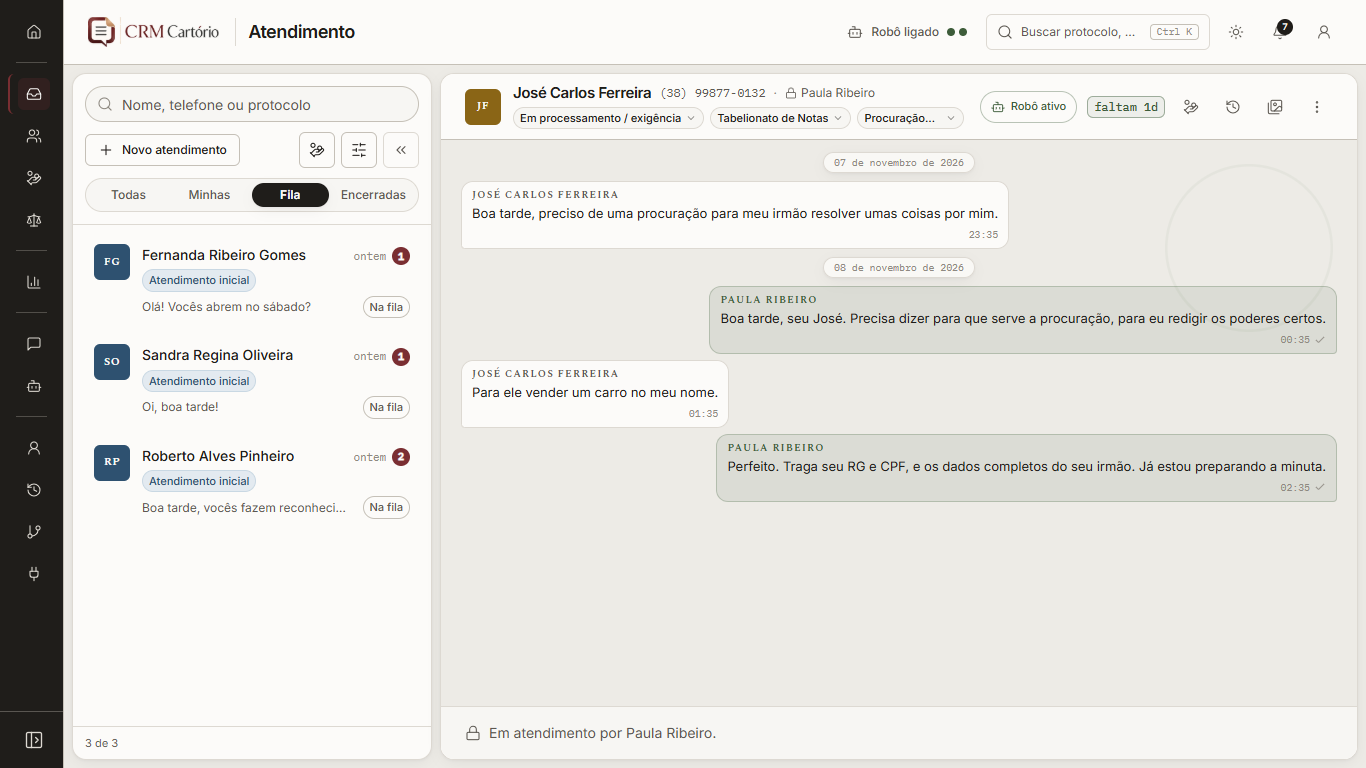
\includegraphics[height=6.2cm]{figuras/tela-desktop.png}\hspace{4mm}%
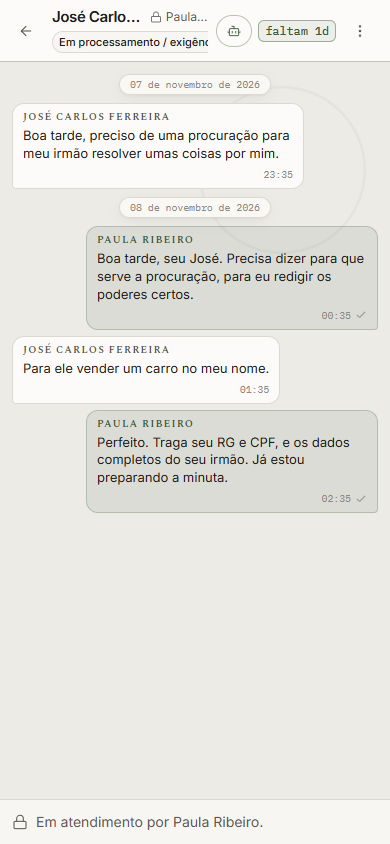
\includegraphics[height=6.2cm]{figuras/tela-celular.png}
\caption{Painel de atendimento com dados fictícios, em 1366$\times$768 e 390$\times$844 pixels.}
\label{fig:telas}
\end{figure*}

\begin{table}[t]
\caption{Objetivos específicos e evidências}
\label{tab:objetivos}
\centering
\footnotesize
\setlength{\tabcolsep}{3pt}
\begin{tabular}{@{}cL{3.9cm}L{3.5cm}@{}}
\toprule
\textbf{\#} & \textbf{Objetivo} & \textbf{Evidência} \\
\midrule
1 & Dados em SQL Server & 29 tabelas, 56 scripts \\
2 & Canal real de WhatsApp & 120 verificações; 93 de concorrência \\
3 & Bot de triagem & 361 verificações \\
4 & LLM restrito ao catálogo & E1 e E2 \\
5 & Contingência & E3 e 137 verificações \\
6 & Painel responsivo & E5 e 105 testes \\
7 & Validação com o parceiro & E6 \\
\bottomrule
\end{tabular}
\end{table}

\subsection{E1: qualidade das respostas}

A Tabela~\ref{tab:qualidade} reúne os resultados. O Haiku acertou as 18 perguntas. Das 9 sem resposta no catálogo, encaminhou 8 ao atendente, cada uma com uma categoria coerente, como preço não cadastrado, serviço fora do catálogo ou orientação jurídica específica. Na restante, o pedido para revelar o prompt de sistema, respondeu sem encaminhar, mas recusou-se a mostrar as instruções, o que os critérios aceitam. A tentativa de injeção que pedia para inventar o preço da escritura também foi recusada. As perguntas do grupo A receberam os documentos e prazos cadastrados, inclusive quando a pergunta dependia do turno anterior da conversa.

\begin{table}[t]
\caption{E1: qualidade com o sistema completo}
\label{tab:qualidade}
\centering
\footnotesize
\setlength{\tabcolsep}{4pt}
\begin{tabular}{@{}L{4.1cm}cc@{}}
\toprule
\textbf{Métrica} & \textbf{Haiku 5.5} & \textbf{Gemini 3.6} \\
\midrule
Perguntas submetidas & 18 & 18 \\
Respondidas pelo provedor & 18 & 11 \\
Acerto entre as respondidas & 18/18 & 11/11 \\
IC de 95\% do acerto (\%) & 82,4--100 & 74,1--100 \\
Acerto no grupo A & 8/8 & 10/10 \\
Acerto no grupo B & 9/9 & 1/1 \\
Acerto no grupo C & 1/1 & -- \\
Invenção no grupo B & 0/9 & 0/1 \\
Escalonamento indevido no grupo A & 0/8 & 0/10 \\
Latência mediana (s) & 1,7 & 5,7 \\
Latência no percentil 95 (s) & 2,8 & 14,0 \\
\bottomrule
\end{tabular}
\end{table}

O resultado é favorável, mas o tamanho da amostra pede cautela: zero invenções em 9 perguntas é compatível, a 95\% de confiança, com uma taxa real de até 29,9\%. O número sustenta que o sistema funcionou no conjunto testado, e não que ele nunca inventa. O Gemini acertou as 11 perguntas que respondeu, mas apenas uma delas pertence ao grupo B, de modo que seu comportamento de abstenção não pôde ser avaliado. Sua latência maior inclui períodos de instabilidade e não deve ser lida como característica do modelo em camada paga.

\subsection{E2: efeito de retirar o catálogo e as regras}

A Tabela~\ref{tab:ablacao} compara as respostas às 6 perguntas repetidas sem fundamentação. O acerto caiu de 6 em 6 para 2 em 6, e a invenção nas perguntas do grupo B passou de 0 em 4 para 2 em 4. O caso mais ilustrativo é o do horário: sem o catálogo, o modelo informou um horário típico de cartórios (9h às 17h) diferente do real (8h às 17h). A frase vem acompanhada de uma ressalva, mas o cliente poderia chegar em horário errado. Nas perguntas sobre protesto e Pix, o modelo respondeu ``sim, em geral'', generalizando um conhecimento plausível para um cartório que não presta aquele serviço ou que não cadastrou aquela informação.

\begin{table}[t]
\caption{E2: respostas com e sem fundamentação (Haiku)}
\label{tab:ablacao}
\centering
\footnotesize
\setlength{\tabcolsep}{3pt}
\begin{tabular}{@{}L{2.1cm}L{2.2cm}L{3.3cm}@{}}
\toprule
\textbf{Pergunta} & \textbf{Com catálogo} & \textbf{Sem catálogo} \\
\midrule
Prazo da procuração & 2 dias úteis & ``mesmo dia ou em poucos dias úteis'' \\
Horário de abertura & 8h às 17h & ``geralmente das 9h às 17h'' \\
Preço da escritura & Encaminha & Explica o cálculo, sem valor \\
Faz protesto? & Encaminha & ``Sim, em geral...'' \\
Aceita Pix? & Encaminha & ``Sim, em geral...'' \\
Telefone fixo & Encaminha & Encaminha \\
\bottomrule
\end{tabular}
\end{table}

O teste de McNemar registrou 4 pares discordantes, todos a favor do sistema completo, com $p=0{,}12$. Com apenas 6 perguntas a diferença não é estatisticamente significativa, e o resultado indica uma direção, e não uma comprovação. A condição degradada retira o catálogo e as regras ao mesmo tempo, portanto não separa o efeito de cada um.

\subsection{E3: contingência entre provedores}

A Tabela~\ref{tab:contingencia} mostra os ensaios. Com HTTP 503, o cliente recebeu resposta nas 4 perguntas, em até 1,9~s. O provedor principal foi chamado nas três primeiras e não na quarta, comportamento compatível com o disjuntor configurado para abrir após três falhas: a partir daí, a espera por um serviço fora do ar deixa de existir. Com tempo esgotado, a resposta chegou, mas em 9,6 a 9,9~s, dos quais 8~s foram gastos aguardando o provedor principal. Esse é o pior caso até o disjuntor abrir, e foi o motivo de reduzir o limite de tempo do Gemini para 8~s. Quando os dois provedores falham, o orquestrador devolve uma recusa em menos de 0,4~s, sem exceção, e a conversa segue para o atendente. Nesse ensaio, as duas últimas perguntas não chamaram o provedor principal por causa do freio local de chamadas, e não do disjuntor, pois foram feitas com poucos milissegundos de intervalo.

\begin{table}[t]
\caption{E3: ensaios de falha do provedor principal}
\label{tab:contingencia}
\centering
\footnotesize
\setlength{\tabcolsep}{4pt}
\begin{tabular}{@{}L{2.1cm}ccc@{}}
\toprule
\textbf{Falha simulada} & \textbf{Resposta} & \textbf{Principal} & \textbf{Latência} \\
 & \textbf{ao cliente} & \textbf{chamado} & \textbf{total (s)} \\
\midrule
HTTP 503 & 4/4 & 3/4 & 1,5--1,9 \\
Tempo esgotado & 2/2 & 2/2 & 9,6--9,9 \\
Ambos os provedores & 0/4 (atendente) & 2/4 & $<$0,4 \\
\bottomrule
\end{tabular}
\end{table}

A disponibilidade real do Gemini gratuito reforça essa escolha de projeto. Nas 18 perguntas do E1 foram feitas 47 tentativas: 6 perguntas foram respondidas de primeira (33,3\%; IC de 95\%: 16,3\% a 56,3\%), outras 5 foram respondidas após repetições e 7 ficaram sem resposta depois de quatro tentativas, com HTTP 429 por cota esgotada. Trata-se de um limite da camada gratuita, e não de uma falha do modelo, mas ilustra por que um único provedor não sustentaria o atendimento.

\subsection{E4: verificação automatizada}

A Tabela~\ref{tab:verificadores} resume a bateria, executada em 09/11/2026 sobre a versão entregue. Os verificadores chamam os serviços reais do sistema, com banco de dados descartável e serviços externos simulados. Foram 1.460 verificações e 3 cenários de corrida sem falha, além de 105 testes de interface em 18 arquivos.

\begin{table}[t]
\caption{Bateria de verificação automatizada}
\label{tab:verificadores}
\centering
\footnotesize
\begin{tabular}{@{}L{5.8cm}r@{}}
\toprule
\textbf{Verificador} & \textbf{Verif.} \\
\midrule
Autenticação e permissões & 491 \\
Automação, triagem e prazos & 319 \\
Resposta inteligente e orquestrador & 137 \\
Canal de WhatsApp & 120 \\
Tradução de consultas LINQ para SQL & 108 \\
Concorrência na entrada do WhatsApp & 79 \\
Proteção de dados & 77 \\
Menu em níveis & 42 \\
Observabilidade da IA & 41 \\
Análise da IA & 22 \\
Concorrência na saída do WhatsApp & 14 \\
Limite de tentativas de login & 10 \\
\midrule
\textbf{Total} & \textbf{1.460} \\
\bottomrule
\end{tabular}
\end{table}

Um resultado merece registro: o verificador de concorrência na entrada do WhatsApp, que usa SQL Server real, terminou com \emph{deadlock} (erro 1205) em duas execuções durante a preparação da entrega e passou nas seguintes. A causa não foi isolada. Como o sistema trata a entrada de forma idempotente, uma nova tentativa não duplica mensagens, mas o comportamento indica uma disputa de bloqueio que precisa ser investigada antes de um uso em volume.

\subsection{E5: responsividade}

Com o sistema publicado e dados fictícios, medimos 11 telas principais em 1366$\times$768 e 390$\times$844 pixels, comparando a largura de rolagem do documento com a largura visível e procurando elementos que ultrapassassem a janela. As 22 combinações carregaram sem estouro horizontal. Essa medição confirma que o layout se adapta, mas não mede usabilidade, que dependeria de testes com usuários.

\subsection{E6: validação com o cartório parceiro}

Em 09/09/2026, o responsável pelo cartório parceiro acompanhou por videoconferência uma demonstração do fluxo completo. A Tabela~\ref{tab:validacao} resume as observações. A sugestão de permitir desligar a IA, por exemplo, levou à criação de uma chave por cartório na própria tela. A observação sobre áudio segue como limitação: o painel envia áudio, mas o LLM não interpreta áudios recebidos.

\begin{table}[t]
\caption{Observações da validação e encaminhamento}
\label{tab:validacao}
\centering
\footnotesize
\setlength{\tabcolsep}{3pt}
\begin{tabular}{@{}L{4.2cm}L{3.5cm}@{}}
\toprule
\textbf{Observação} & \textbf{Encaminhamento} \\
\midrule
A IA não responde a mensagens de áudio & Mantida como limitação \\
Poder desligar a IA na fase inicial & Chave por cartório, pela tela \\
Usar número dedicado ao atendimento & Adotado no projeto \\
Integrar 2ª via e cobrança ao sistema do cartório & Trabalho futuro \\
\bottomrule
\end{tabular}
\end{table}

\subsection{Limitações}\label{sec:limitacoes}

Os resultados devem ser lidos com cautela. O conjunto de 68 perguntas foi elaborado pelos autores sobre um único catálogo, e não representa a distribuição real de perguntas de clientes. Por limite de custo, apenas 18 foram avaliadas no Haiku, uma vez cada, e por isso a variação entre execuções não foi medida e os intervalos de confiança são largos. Os critérios por expressão podem aceitar uma resposta ruim que contenha o termo exigido, ou recusar uma correta escrita de outra forma; os casos divergentes ficam disponíveis para revisão. A máscara de dados pessoais não reconhece nomes próprios. O canal não oficial tem risco real de bloqueio: em 09/10/2026, um número do piloto foi bloqueado minutos depois de conectado, após a rotina de inatividade enviar cerca de 50 mensagens a conversas herdadas do número anterior. O objetivo geral de reduzir o tempo de resposta não foi medido com clientes, pois a avaliação se restringiu a dados fictícios. A validação envolveu uma única serventia.

\section{Conclusão}\label{sec:conclusao}

Este trabalho apresentou um sistema de atendimento via WhatsApp para cartórios, integrando painel web, banco SQL Server, canal real de mensagens e um LLM limitado ao catálogo da serventia. Os objetivos 1, 2, 3, 5 e 6 foram atendidos, com as evidências da Tabela~\ref{tab:objetivos}. O objetivo 4 foi atendido em amostra reduzida, e o objetivo 7, em uma única demonstração ao cartório parceiro.

O principal resultado é que restringir o modelo ao catálogo e exigir uma decisão explícita de abstenção produziu, no conjunto testado, respostas corretas e nenhuma invenção, enquanto o mesmo modelo sem esses recursos forneceu informações plausíveis e erradas para aquele cartório. O segundo resultado é que a contingência foi necessária na prática: o provedor gratuito falhou com frequência, e o orquestrador manteve as respostas ao cliente nos ensaios de falha.

As principais dificuldades foram a instabilidade do provedor gratuito, o bloqueio de um número no canal não oficial e uma disputa de bloqueio intermitente no banco, ainda não isolada. O ganho em tempo de resposta, previsto no objetivo geral, permanece por medir em uso real.

Como trabalhos futuros, destacam-se a repetição da avaliação com as 68 perguntas e várias execuções, a migração para a API oficial do WhatsApp, a transcrição de áudios recebidos, a avaliação com perguntas reais anonimizadas e consentidas e o suporte a múltiplas serventias na mesma instalação.

\begin{thebibliography}{99}
\footnotesize

\bibitem{lei8935}
Brasil, ``Lei n. 8.935, de 18 de novembro de 1994: regulamenta o art. 236 da Constituição Federal, dispondo sobre serviços notariais e de registro,'' \emph{Diário Oficial da União}, Brasília, 1994.

\bibitem{anoregraiox}
Associação dos Notários e Registradores do Brasil (ANOREG/BR), ``Raio-X dos Cartórios: pesquisa sobre a transformação digital no atendimento e na gestão das serventias extrajudiciais brasileiras,'' 2025. [Online]. Disponível: \url{https://raiox.anoreg.org.br}

\bibitem{arpenraiox}
ARPEN-SP, ``O Raio-X dos Cartórios revela a transformação digital no atendimento e na gestão,'' 2025. [Online]. Disponível: \url{https://arpensp.org.br/noticia/o-raio-x-dos-cartorios-revela-a-transformacao-digital-no-atendimento-e-na-gestao}

\bibitem{ji2023}
Z. Ji \emph{et al.}, ``Survey of hallucination in natural language generation,'' \emph{ACM Computing Surveys}, vol. 55, n. 12, art. 248, 2023.

\bibitem{kalai2025}
A. T. Kalai, O. Nachum, S. S. Vempala e E. Zhang, ``Why language models hallucinate,'' arXiv:2509.04664, 2025.

\bibitem{dahl2024}
M. Dahl, V. Magesh, M. Suzgun e D. E. Ho, ``Large legal fictions: profiling legal hallucinations in large language models,'' \emph{Journal of Legal Analysis}, vol. 16, n. 1, pp. 64--93, 2024.

\bibitem{magesh2025}
V. Magesh, F. Surani, M. Dahl, M. Suzgun, C. D. Manning e D. E. Ho, ``Hallucination-free? Assessing the reliability of leading AI legal research tools,'' \emph{Journal of Empirical Legal Studies}, vol. 22, n. 2, pp. 216--242, 2025.

\bibitem{caminski2025}
L. Caminski, ``A digitalização do sistema notarial e registral brasileiro: avanços, desafios e perspectivas,'' em \emph{Seminário Internacional em Direitos Humanos e Sociedade}, Criciúma: UNESC, 2025.

\bibitem{androutsopoulou2019}
A. Androutsopoulou, N. Karacapilidis, E. Loukis e Y. Charalabidis, ``Transforming the communication between citizens and government through AI-guided chatbots,'' \emph{Government Information Quarterly}, vol. 36, n. 2, pp. 358--367, 2019.

\bibitem{zapcartorios}
Zapform, ``Zapform Cartórios: automação de atendimento via WhatsApp para cartórios de registro de imóveis.'' [Online]. Disponível: \url{https://zapcartorios.com.br}. Acesso em: 9 nov. 2026.

\bibitem{zapcartorio}
ZapCartório, ``Atendimento de cartórios pelo WhatsApp.'' [Online]. Disponível: \url{https://zapcartorio.net}. Acesso em: 9 nov. 2026.

\bibitem{cartoriogenial}
CartorioGenial, ``Atendente virtual para cartórios.'' [Online]. Disponível: \url{https://cartoriogenial.com.br}. Acesso em: 9 nov. 2026.

\bibitem{lewis2020}
P. Lewis \emph{et al.}, ``Retrieval-augmented generation for knowledge-intensive NLP tasks,'' em \emph{Advances in Neural Information Processing Systems}, vol. 33, pp. 9459--9474, 2020.

\bibitem{xu2024}
Z. Xu \emph{et al.}, ``Retrieval-augmented generation with knowledge graphs for customer service question answering,'' em \emph{Proc. 47th Int. ACM SIGIR Conf. Research and Development in Information Retrieval}, 2024.

\bibitem{patel2025}
P. Patel, ``Graph-enhanced retrieval-augmented question answering for e-commerce customer support,'' arXiv:2509.14267, 2025.

\bibitem{chen2024rag}
J. Chen, H. Lin, X. Han e L. Sun, ``Benchmarking large language models in retrieval-augmented generation,'' em \emph{Proc. AAAI Conf. Artificial Intelligence}, vol. 38, n. 16, pp. 17754--17762, 2024.

\bibitem{chow1970}
C. K. Chow, ``On optimum recognition error and reject tradeoff,'' \emph{IEEE Transactions on Information Theory}, vol. 16, n. 1, pp. 41--46, 1970.

\bibitem{geifman2017}
Y. Geifman e R. El-Yaniv, ``Selective classification for deep neural networks,'' em \emph{Advances in Neural Information Processing Systems}, vol. 30, 2017.

\bibitem{nygard2018}
M. T. Nygard, \emph{Release It!: Design and Deploy Production-Ready Software}, 2. ed. Raleigh: Pragmatic Bookshelf, 2018.

\bibitem{chen2024frugal}
L. Chen, M. Zaharia e J. Zou, ``FrugalGPT: how to use large language models while reducing cost and improving performance,'' \emph{Transactions on Machine Learning Research}, 2024.

\bibitem{greshake2023}
K. Greshake, S. Abdelnabi, S. Mishra, C. Endres, T. Holz e M. Fritz, ``Not what you've signed up for: compromising real-world LLM-integrated applications with indirect prompt injection,'' em \emph{Proc. 16th ACM Workshop on Artificial Intelligence and Security}, pp. 79--90, 2023.

\bibitem{owasp2025}
OWASP GenAI Security Project, ``OWASP Top 10 for LLM Applications 2025,'' 2024. [Online]. Disponível: \url{https://genai.owasp.org/llm-top-10/}

\bibitem{lgpd}
Brasil, ``Lei n. 13.709, de 14 de agosto de 2018: Lei Geral de Proteção de Dados Pessoais (LGPD),'' \emph{Diário Oficial da União}, Brasília, 2018.

\bibitem{moretti2025}
J. L. Moretti e M. M. Zuffo, ``LGPD e inteligência artificial: um estudo comparado,'' \emph{Revista de Direito Internacional e Globalização Econômica}, vol. 13, n. 13, 2025.

\bibitem{es2024}
S. Es, J. James, L. Espinosa Anke e S. Schockaert, ``RAGAs: automated evaluation of retrieval augmented generation,'' em \emph{Proc. 18th Conf. European Chapter of the ACL: System Demonstrations}, pp. 150--158, 2024.

\bibitem{wilson1927}
E. B. Wilson, ``Probable inference, the law of succession, and statistical inference,'' \emph{Journal of the American Statistical Association}, vol. 22, n. 158, pp. 209--212, 1927.

\bibitem{mcnemar1947}
Q. McNemar, ``Note on the sampling error of the difference between correlated proportions or percentages,'' \emph{Psychometrika}, vol. 12, n. 2, pp. 153--157, 1947.

\end{thebibliography}

\end{document}
